% first example chapter
% @author Jan Robert Rösler 
%
\chapter{Auswertung und Szenarien}
In diesem Kapitel wird der Traningsprozess analysiert und kritisch Bewertet, zudem wird das entworfene neuronale Steuerungssystem einem Test unterzogen. Verschiedene Fahrszenarien werden untersucht, zum Schluss bietet eine grafische Auswertung einen Einblick in die Perspektive aus Sicht des neuronalen Netzes.

\section{Training}
Das Fine-Tuning wurde mit den im vorangegangenem Kapitel festgelegten Konfigurationen durchgeführt. In diesem Abschnitt erfolgt eine Betrachtung des erfolgten Tranings. In Abbildung:~\ref{img:loss} sind Traningsfehler und Validierungsfehler (y-Achse) über $100$ Epochen (x-Achse) dargestellt. 

\begin{figure}[h]
	\centering
	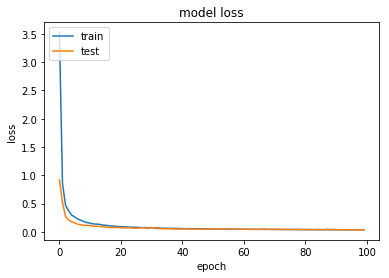
\includegraphics[scale=0.7]{figures/loss.png}
	\caption{Traningsfehler (train) und Validierungsfehler (val) über 100 Epochen}
	\label{img:loss}
\end{figure}

Festzustellen ist, dass beide Fehlerwerte sich zunächst stark fallend $0.0$ annähren und zwischen den Epochen $20-25$ und $100$ gleichbleibend $0.0$ zu sein scheinen. Aufgrund der Start-Traningsfehler von etwa $3.5$ lassen sich sehr kleine Werte nicht grafisch beurteilen. Ein direkter Blick auf die Fehlerwerte zeigt, dass beide sich im Bereich \num{10e-2} befinden mit dem Besten Validierungsfehler von $0.0344$ in Epoche $197$. Es besteht keine ausgeprägte Divergenz zwischen Trainings- und Validierungsfehler, das ist positiv zu beurteilen.\\
Bei kritischer Betrachtung muss angemerkt werden, dass die Regressionkurve, im konkreten Fall die Annäherung des Lenkwinkels, sehr rapide fällt. Dieses kann Zeichen eines Overfittings sein. Die Bilder der Teststrecke könnten in der Menge zu homogen sein, die Teststrecke ist im Angesicht der dort aufgenommenen Bildermenge relativ kurz. Aufgrund der räumlichen Abgeschlossenheit der Teststrecke gibt es dazu wenig Variabilität im Bildhintergrund, das könnte die Gleichartigkeit der Bilder verstärken.\\
Allerdings ist die schnelle Konvergenz nicht zwingend negativ anzumerken, das neuronale Netz war schließlich schon mit derselben Aufgabe auf einer ähnlichen Bildermenge trainiert worden. Dazu kommt, dass nur ein Teil der Layer überhaupt für das Traning, also eine Veränderung der Gewichte, freigegeben war. Im Angesicht dieser Umstände, können die Fehlerkurven in Abbildung~\ref{img:loss} auch für eine schnelle, effiziente Anpassung der Gewichte des letzten Residual-Blocks stehen.




\section{Metriken}

tabelle machen


Auch Geschwindigkeiten beachten, Carolo-Net performt bis 1.2 m/s
\section{Testfahrten}

1. Auto mit Dronet 
2. Auto mit adaptiertem Netz
3. Auto mit Netz des aktuellen Carolo-Cup Teams 

\section{Sonderszenarien}

\paragraph{Kreuzung}

\paragraph{Fahrbahn wiederfinden}

Performance (Rechenzeit) bei prediction auf dem Fahrzeug


- Findet das Auto auf die Strecke zurück? Schräg ansetzen und autonomen Modus starten
(Zeigt ob Strecke nur auswensig gelernt oder nicht, da  diese blickwinkel nicht im Trainingsset enthalten sind)

\section{Saliency}

zitieren woher der code kommt !''
- Saliency Besipiele Zeigen was für Features erlernt wurden. (Eventuell auch von vorangegangenen Layern)

-Vielleicht noch ein Szenario in dem das Validation set exra schwer (Artefakte) gemacht wurde

\note{Auf die Problematik mit Testsetgröße eingehen, kleines set daher nur letzter blockj trainiert etc....}



Kurzer Blick auf  Self driving car steering angle4 prediction und berkeley (large scale video sets) (vielleicht auchSPÄTER)